\documentclass[xcolor=table, 9pt]{beamer}
%\usetheme{Copenhagen}
\usetheme{Darmstadt}

\definecolor{Red}{rgb}{0.674509804, 0.223529412,0.223529412} % UBC Red (primary)
\definecolor{mavi}{rgb}{0,0.1568,0.3019}

\usecolortheme[named=mavi]{structure}

\usepackage{graphicx} % Allows including images
\usepackage{booktabs} % Allows the use of \toprule, \midrule and \bottomrule in tables
\usepackage[utf8]{inputenc}
\usepackage{animate}
\usepackage[math]{iwona}
\usepackage[T1]{fontenc}
\usepackage{makecell}
\usepackage{graphicx}
\usepackage{wasysym}
\usepackage{setspace}
\usepackage{listings}
\usepackage{color}
\usepackage{stackrel,amssymb}


\renewcommand\theadalign{cb}
\renewcommand\theadfont{\bfseries}
\renewcommand\theadgape{\Gape[2pt]}
\renewcommand\cellgape{\Gape[2pt]}

\newcommand*{\vimage}[1]{\vcenter{\hbox{\includegraphics[scale=0.08]{#1}}}}
\newcommand*{\vpointer}{\vcenter{\hbox{\scalebox{2}{\Huge\pointer}}}}


\colorlet{mycolor}{Red!80!black}

%----------------------------------------------------------------------------------------
%	FOOTER
%----------------------------------------------------------------------------------------

\makeatother
\setbeamertemplate{footline}
{
  \leavevmode%
  \hbox{%
  \begin{beamercolorbox}[wd=.5\paperwidth,ht=2.25ex,dp=1ex,right]{author in head/foot}%
    \usebeamerfont{author in head/foot}\insertshortauthor\hspace*{3em}
  \end{beamercolorbox}%
  \begin{beamercolorbox}[wd=.5\paperwidth,ht=2.25ex,dp=1ex,left]{title in head/foot}%
    \hspace*{3em}\usebeamerfont{title in head/foot}\insertshorttitle\hspace{4.3cm}
    \insertframenumber{} / \inserttotalframenumber\hspace{1ex}
  \end{beamercolorbox}}%
  \vskip0pt%
}
\makeatletter
\setbeamertemplate{navigation symbols}{}


%----------------------------------------------------------------------------------------
%	TITLE PAGE
%----------------------------------------------------------------------------------------

\title[Thesis]{Bluetooth-WIFI Communication Car}

\author{Author: Mehmetcan Güleşçi} % Your name
\institute[CMPE 491]
{
Istanbul Bilgi University \\
\medskip
\textit{Computer Engineering} 
}
\date{\today} % Date, can be changed to a custom date



\begin{document}


\begin{frame}
\titlepage 
\end{frame}


   \setbeamercolor{section in toc shaded}{use=structure,fg=structure.fg}
   \setbeamercolor{section in toc}{fg=mycolor}
   \setbeamercolor{section in toc shaded}{use=structure,fg=structure.fg}
   \setbeamercolor{section in toc}{fg=mycolor}
   \setbeamercolor{section in toc shaded}{use=structure,fg=structure.fg}


%----------------------------------------------------------------------------------------
%	PRESENTATION SLIDES
%----------------------------------------------------------------------------------------

%------------------------------------------------

\begin{frame}{ABSTRACT}
\begin{itemize}
\item Using of smartphones
\item Development of smartphones in terms of low cost robots.
\item About project
\end{itemize}
\end{frame}


%----------------------------------------


\begin{frame}
\begin{figure}
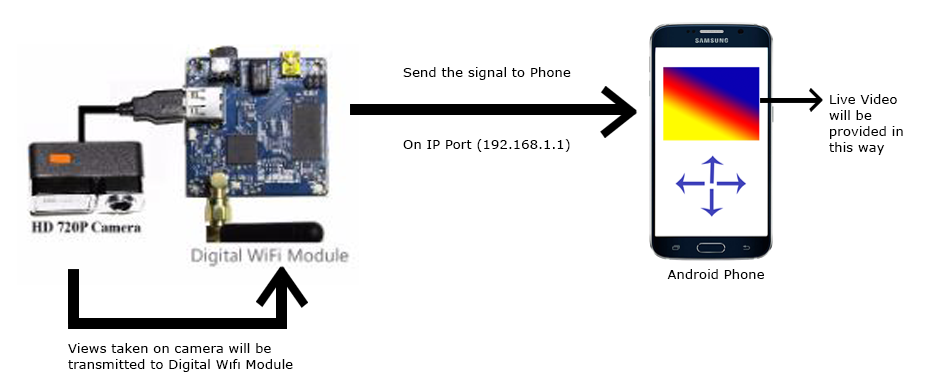
\includegraphics[width=1.08\linewidth]{wificom.png}
\caption{WIFI Communication}
\end{figure}
\end{frame}


%----------------------------------------


\begin{frame}
\begin{figure}
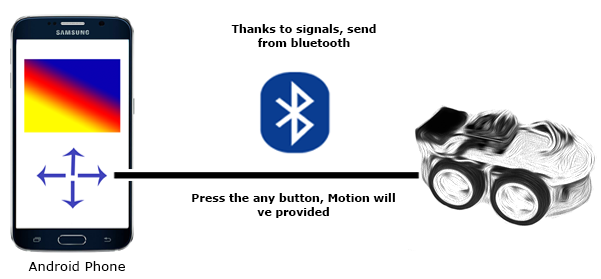
\includegraphics[width=1.05\linewidth]{astractblue.png}
\caption{Bluetooth Communication}
\end{figure}
\end{frame}


%----------------------------------------


\begin{frame}{INTRODUCTION}
\begin{itemize}
\item A benefit of having a Bluetooth connection.
\item Two parts of communication
\end{itemize}
\end{frame}


%----------------------------------------


\begin{frame}
\begin{figure}
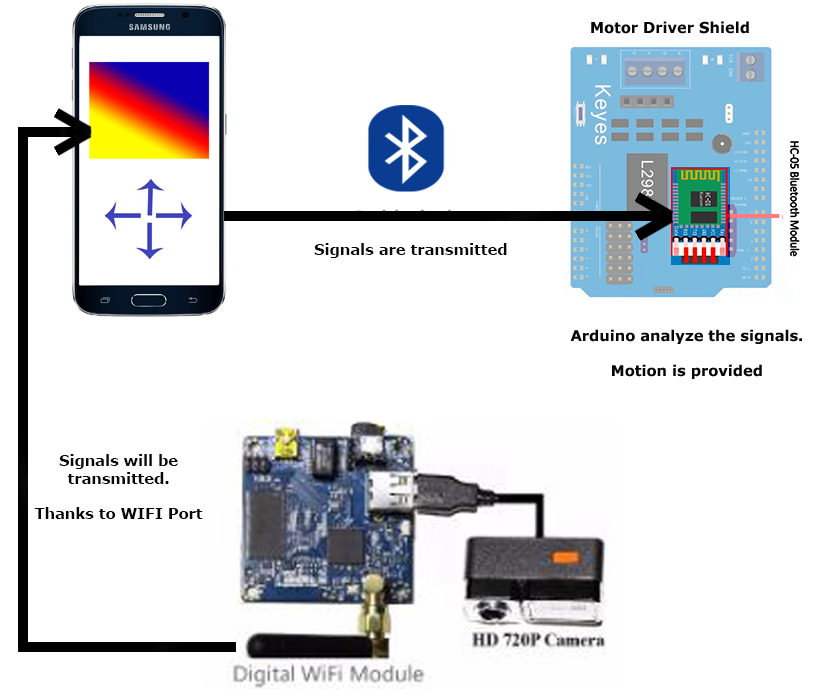
\includegraphics[width=0.70\linewidth]{bluewifisheme.png}
\caption{All Parts of Communications}
\end{figure}
\end{frame}


%----------------------------------------


\begin{frame}{Communication Between Devices}
\begin{table}
\begin{tabular}{ |c| c | c | c | c |}
\hline
\thead{From/To \\ Android} & \thead{From/To \\ HD Camera} & \thead{On \\ WIFI Module} & \thead{On - From/To \\ Motor Shield \\ (UNO R3)} & \thead{On \\ Bluetooth}\\ \hline

\makecell{Signal to \\ Android \\ from \\HD Cam (1)} &  \makecell{Signal from \\ HD Cam \\ to Android (2)}  & \color{mavi}\Huge $\bullet$ & \color{mavi}\Huge $\bullet$ &   \\ \hline

\makecell{Signal from \\ Android \\ to\\ Motor \\Shield (3)} &    &  & \makecell{Signal to \\Motor Shield \\ from Android (4)} & \color{mavi}\Huge $\bullet$   \\ \hline
\end{tabular}
\caption{Communication Tables}
\end{table}
\end{frame}


%----------------------------------------
	

\begin{frame}{Objectives}
\begin{itemize}
\item[1] To enable inserting Arduino Code to give first motion to the car.
\item[2] To enable Android buttons to control the Car as remoted.
\item[3] To enable getting live view on the HD Cam by using WIFI Module and to display the robot eyes on Android Screen.
\end{itemize}
\end{frame}


%----------------------------------------


\begin{frame}{Requirements}
\begin{table}[h]
\centering 
\begin{tabular}{|c|c|}
 \hline
 \textbf{\emph{\cellcolor{red!27}{\small Number}}} & \textbf{\emph{\cellcolor{red!27}{\small Needed}}}	\\ [0.5ex] \hline
 1 &{\small  UNO R3} \\  \hline
 1 & {\small L298P Motor Shield} \\  \hline
 1 & {\small Digital WIFI Module} \\  \hline
 1 & {\small HD Camera} \\  \hline
 1 & {\small HC05 Bluetooth Module} \\ \hline
 1 & {\small DC Motors} \\
 \hline
\end{tabular}
\caption{Requirements}
\label{table:1}
\end{table}
These are necessary parts which I will use for this robot. Now I want to talk about them.
\end{frame}


%----------------------------------------


\begin{frame}{Arduino Uno R3}
\begin{columns}[c] 
\column{.45\textwidth} % Left column and width

\begin{itemize}
\item[] \textbf{What is Arduino?}\\~\\
\item[] This unit is a micro controller that makes what you want when you want it or controls physical inputs with various sensors and converts these inputs into the desired output. 
\end{itemize}
\column{.5\textwidth} % Right column and width
\begin{figure}
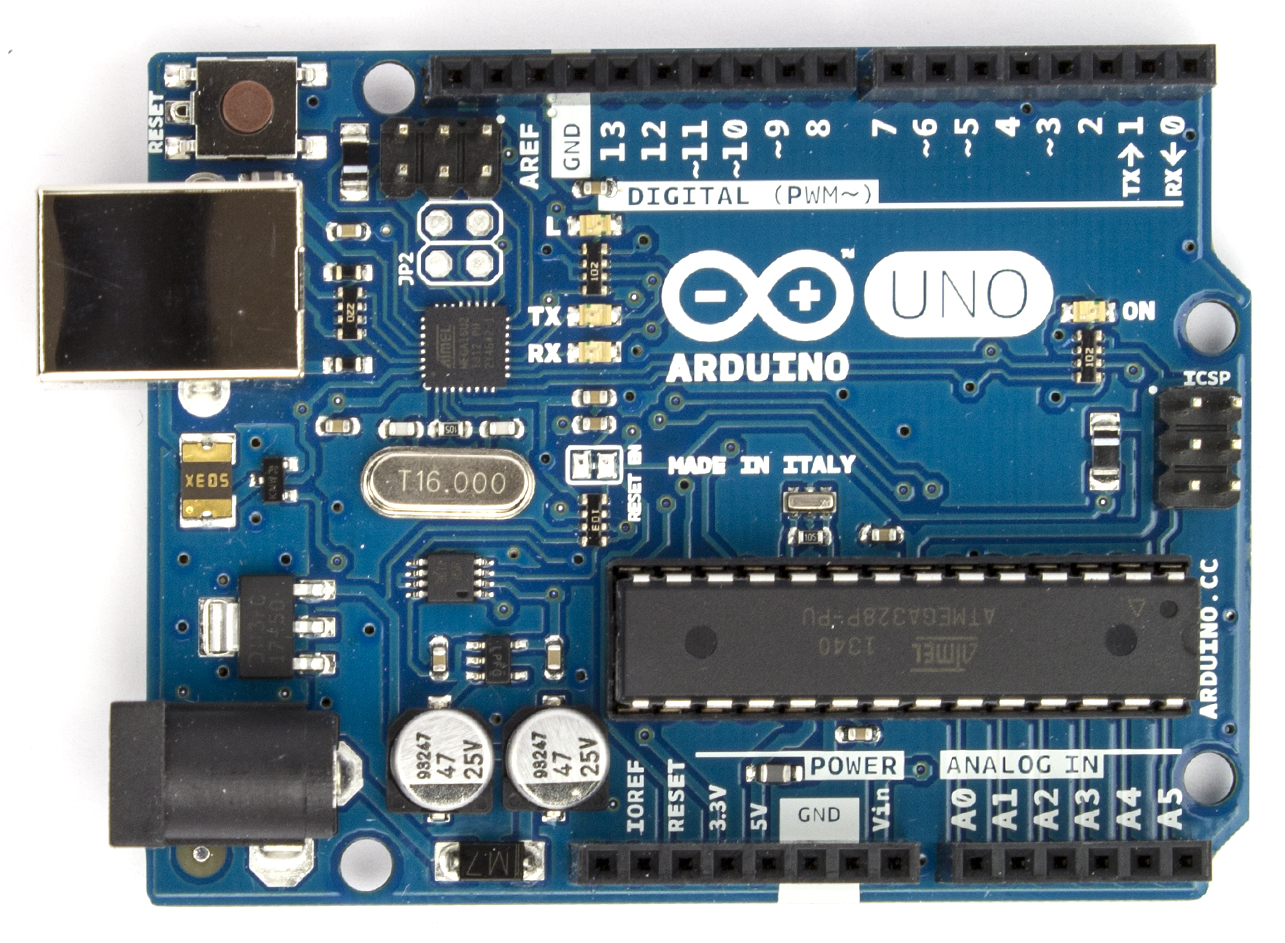
\includegraphics[width=0.7\linewidth]{arduino.png}
\caption{Uno R3}
\end{figure}
\end{columns}
\end{frame}


%----------------------------------------


\begin{frame}{Arduino Uno R3}
\begin{itemize}
\item Like your computer's processor.
\item Like your brain.
\item Easy to use
\item Thanks to sensors and activators on Arduino, you can do whatever you want.
\item This requires only a little electronic knowledge and a little programming knowledge.
\item Writing a program with Arduino is simpler.
\end{itemize}
\end{frame}


%----------------------------------------


\begin{frame}{Arduino Uno R3}
\begin{columns}[c] 
\column{.55\textwidth} % Left column and width
\textbf{Input Outputs}\\~\\
\begin{itemize}
\item[1]Usb cable
\item[2]External power supply (7-12V)
\item[3]Digital pins 3,5,6,9,10,11 PWM
\item[4]Rx (Receive data), Tx (Transmit data)
\item[5]Reset Button 
\item[6]3.3V, 5V, GND 
\end{itemize}
\column{.45\textwidth} % Right column and width
\begin{figure}
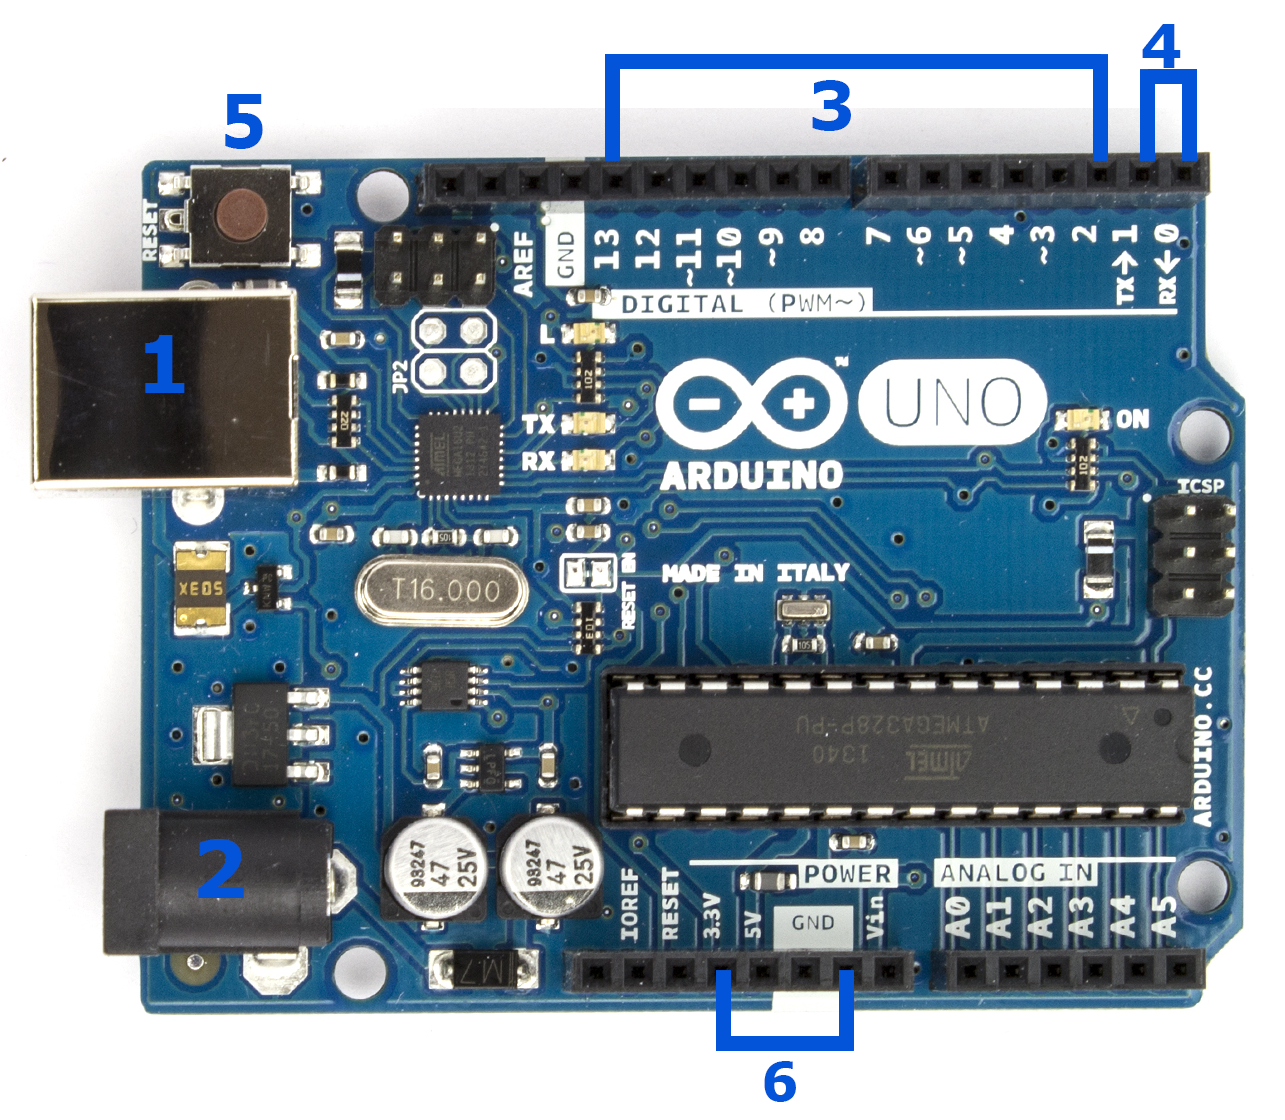
\includegraphics[width=1\linewidth]{arduinoreview.png}
\caption{Arduino detailed review}
\end{figure}
\end{columns}
\end{frame}


%----------------------------------------


\begin{frame}{L298P Motor Shield}
\begin{columns}[c] 
\column{.60\textwidth}
\begin{itemize}
\item Full-bridge motor driver 
\item Take Arduino's data.
\item Directly plugged into the Arduino.
\item Drive two separate 2A DC motors 
\item On board buzzer (D4), you can set the alarm ringtone.
\item Bluetooth interface requires no wiring and you can plug directly.
\item Six analog interfaces (A0, A1, A2, A3, A4, and A5).
\item Seven digital interface that are not occupied (D2, D3, D5, D6, D7, D8, and D9).
\end{itemize}
\column{.40\textwidth}
\begin{figure}
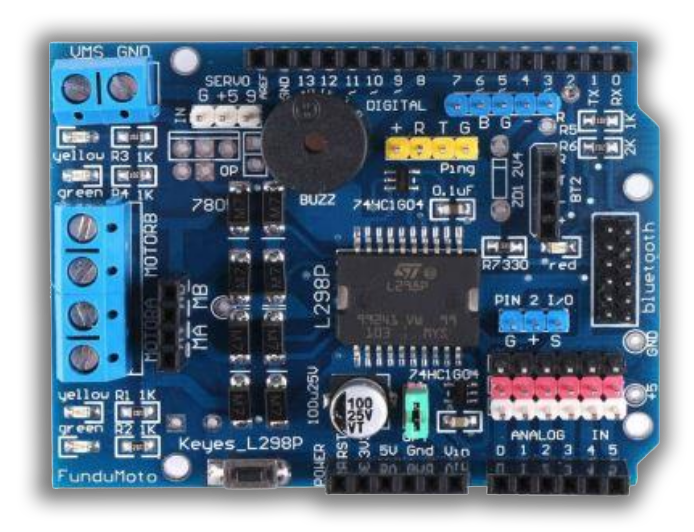
\includegraphics[width=1\linewidth]{l298.png}
\caption{L298P Motor Shield}
\end{figure}
\end{columns}
\end{frame}


%----------------------------------------

\begin{frame}{L298P Motor Shield}
\begin{table}[h]
\centering 
\begin{tabular}{|c|c|c|}
 \hline
 \textbf{\emph{\cellcolor{red!27}{\small Function}}} & \textbf{\emph{\cellcolor{red!27}{\small Channel A Pin}}} & \textbf{\emph{\cellcolor{red!27}{\small Channel B Pin}}}	\\ [0.5ex] \hline
 {\small Direction} & {\small D12} & {\small D13} \\  \hline
 {\small PWM} & {\small D10} & {\small D11}\\ 
 \hline
\end{tabular}
\caption{Shield pin usage table}
\label{table:1}
\end{table}
\end{frame}


%----------------------------------------


\begin{frame}{Digital WIFI Module}
\begin{columns}[c] 
\column{.55\textwidth}
\begin{itemize}
\item Thanks to this card, our Android application will be connected to Cam port by using IP which is in this module. (may be 192.168.1.1)
\item The usb input on it allows us to connect our HD Cam.
\item The cables from the WIFI Module are connected to the relevant parts of the L298P Motor Shield which is integrated on the Arduino. (Just to provide a power etc. GND-5V )
\item The connection will be provided between android phone and camera on the WIFI Module's IP address.
\end{itemize}
\column{.45\textwidth}
\begin{figure}
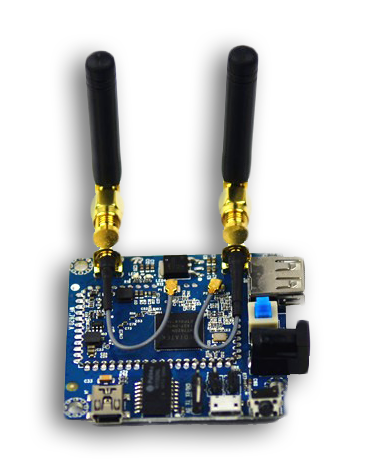
\includegraphics[width=1\linewidth]{wifi.png}
\caption{Digital WIFI Module}
\end{figure}
\end{columns}
\end{frame}


%----------------------------------------


\begin{frame}{Digital WIFI Module}
\begin{figure}
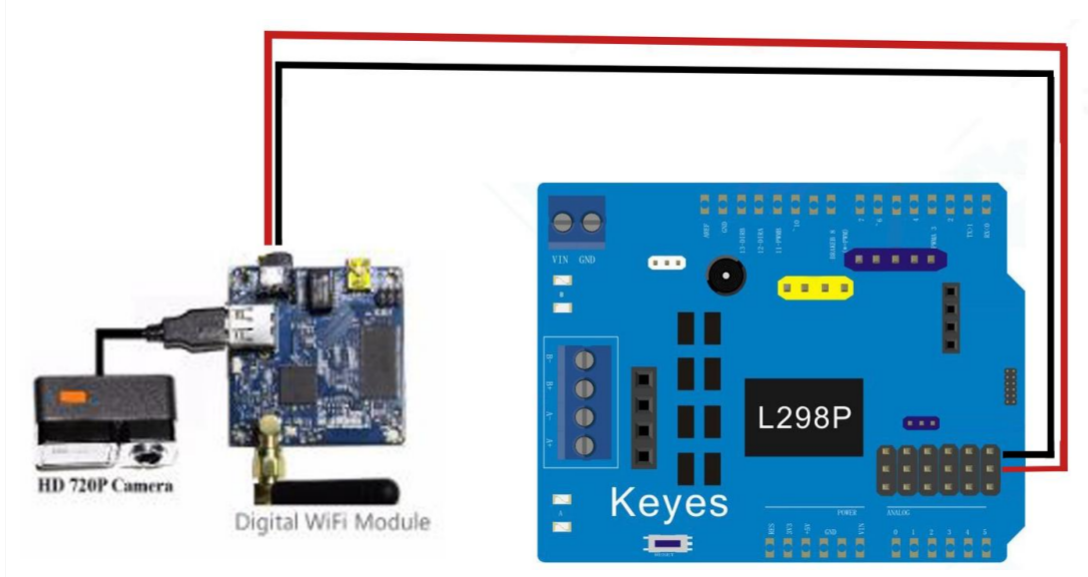
\includegraphics[width=1\linewidth]{connectwifi.png}
\caption{Digital WIFI Module and L298P Motor Shield}
\end{figure}
\end{frame}

%----------------------------------------


\begin{frame}{HD Camera}
\begin{columns}[c] 
\column{.55\textwidth}
\begin{block}{Using HD Cam}
It will be possible to transfer live video to the phone with the HD camera when the necessary operation is done thanks to the usb connection which is connected to WIFI Module.
\end{block}
\column{.45\textwidth}
\begin{figure}
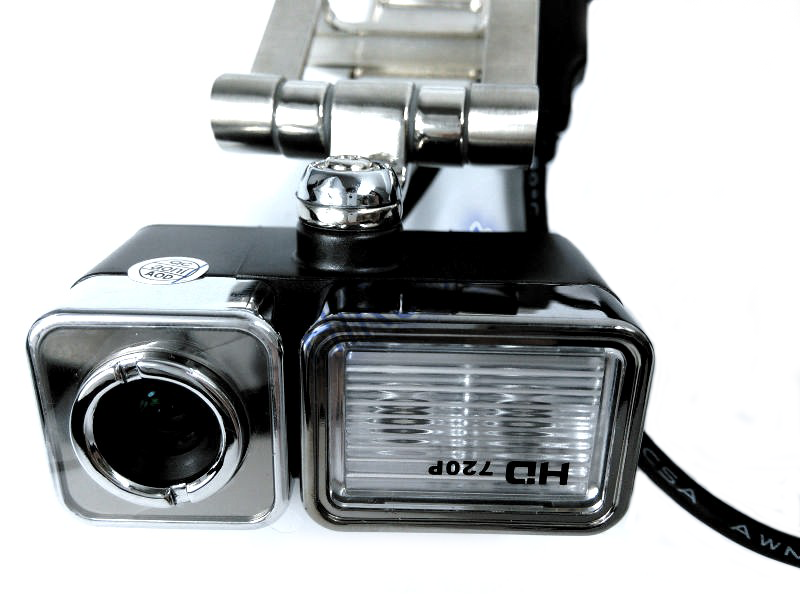
\includegraphics[width=1\linewidth]{camtemiz.png}
\caption{HD Cam}
\end{figure}
\end{columns}
\end{frame}


%----------------------------------------


\begin{frame}{Bluetooth Module}
\begin{columns}[c] 
\column{.55\textwidth}
\begin{itemize}
\item There are 4 pins on VCC, GND, Rx and Tx on the Bluetooth module.
\item From these VCC and GND are used to feed the Uno module
\item This project will be designed as sending data to Bluetooth module when certain button
pressed from user. (figure)
\item The Bluetooth module on Arduino receives the data and send to Arduino through the TX pin
of Bluetooth module (RX pin of Arduino).(figure)
\end{itemize}
\column{.45\textwidth}
\begin{figure}
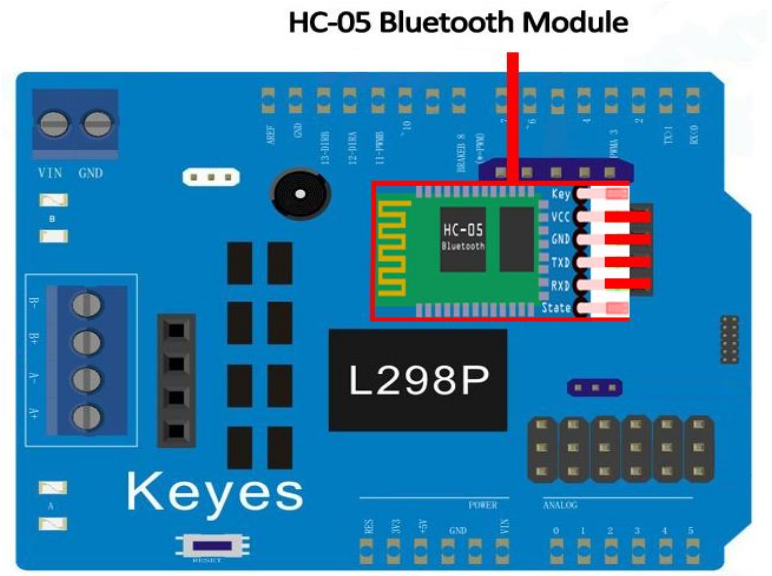
\includegraphics[width=1\linewidth]{blue.png}
\caption{Bluetooth Module on L298P}
\end{figure}
\end{columns}
\end{frame}


%----------------------------------------

\begin{frame}
\begin{figure}
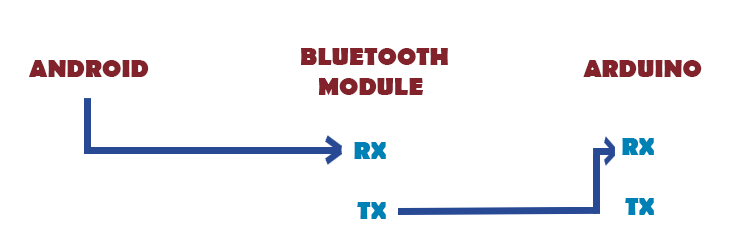
\includegraphics[width=1\linewidth]{bluetsheme.png}
\caption{RX,TX Connection}
\end{figure}
\end{frame}


%----------------------------------------


\begin{frame}{DC Motors}
\begin{columns}[c] 
\column{.55\textwidth}
\textbf{Basic Features}\\~\\
\begin{itemize}
\item The most preferred type of motor
\item Cheap, small and effective. 
\item Various size, shape and power\\~\\ 
\end{itemize}
Now we will explain dc motors in terms of direction, speed, voltage and current.
\column{.45\textwidth}
\begin{figure}
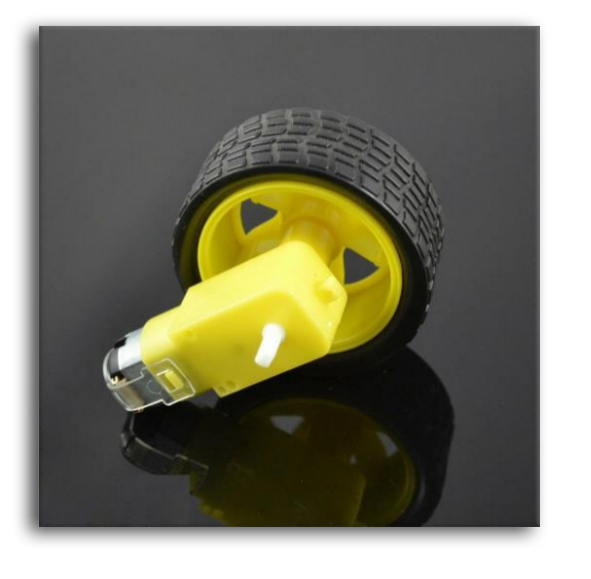
\includegraphics[width=0.85\linewidth]{dcmotor.png}
\caption{DC Motor}
\end{figure}
\end{columns}
\end{frame}



\begin{frame}{DC Motors}
\begin{figure}
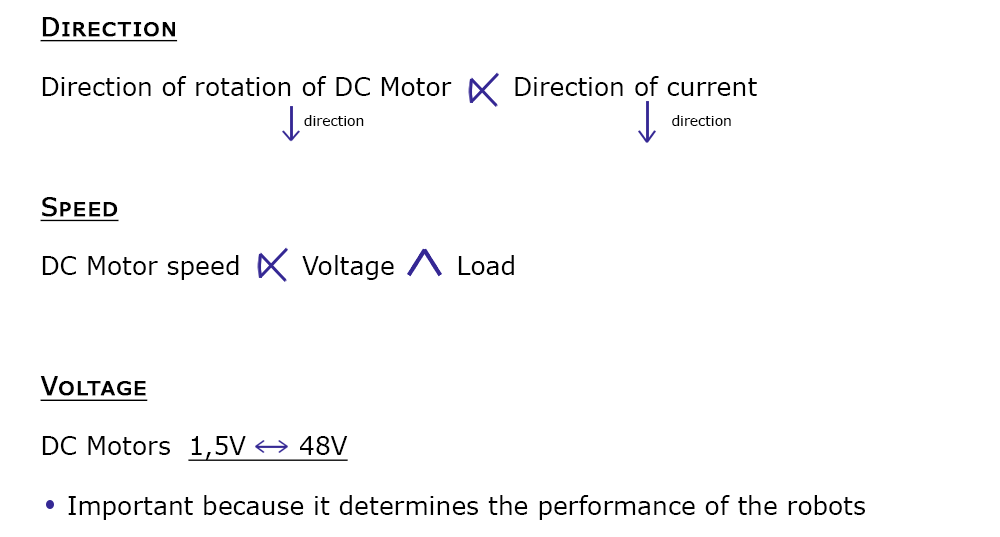
\includegraphics[width=0.9\linewidth]{dsv.png}
\end{figure}
\end{frame}


%----------------------------------------


\begin{frame}{DC Motors}
\begin{figure}
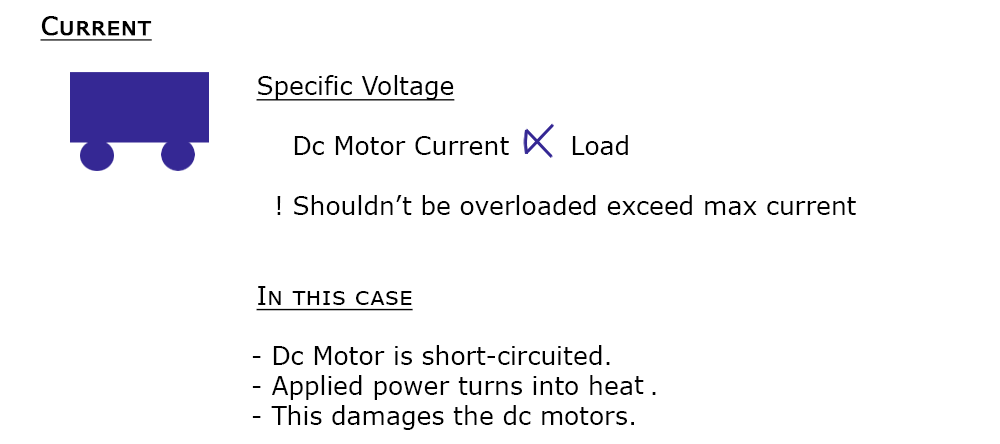
\includegraphics[width=0.9\linewidth]{c.png}
\end{figure}

\begin{figure}
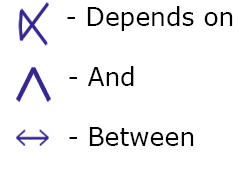
\includegraphics[width=0.10\linewidth]{signs.png}
\end{figure}

\end{frame}


%----------------------------------------


\begin{frame}{DC Motors}
\begin{figure}
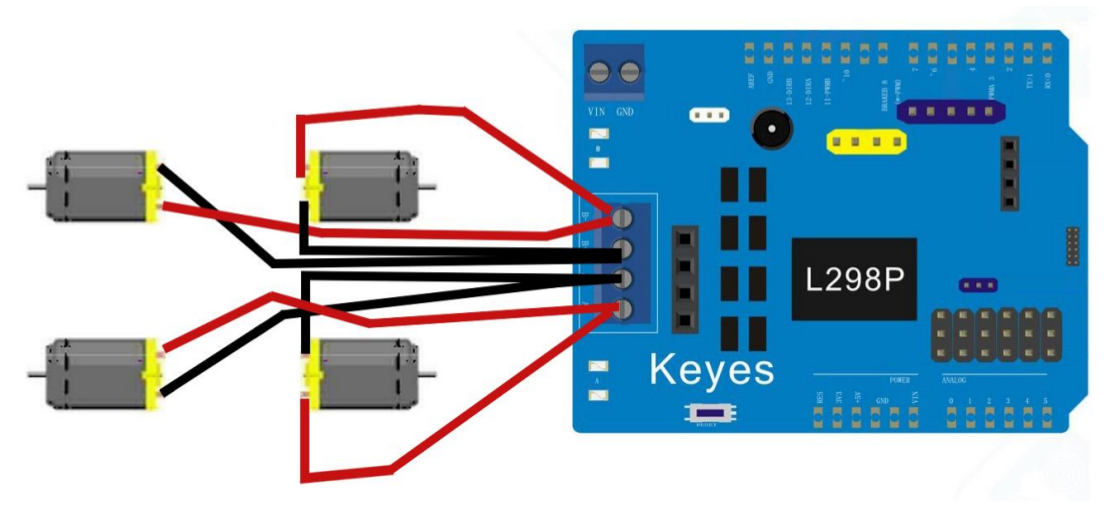
\includegraphics[width=1\linewidth]{connectl298.png}
\caption{Connect L298P to DC Motors}
\end{figure}
\end{frame}

%----------------------------------------

\begin{frame}{Car Building Process}
On the hardware side, the first step is to mount the dc motors which are wired, to the chassis.\\
\begin{figure}[h]
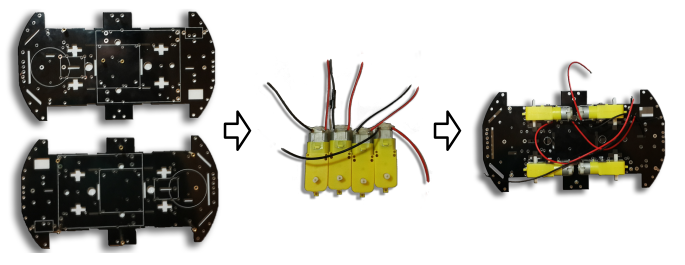
\includegraphics[width=1\linewidth]{build1.png}
\caption{Building Process 1}
\end{figure}
\end{frame}

\begin{frame}{Car Building Process}
The second step is to connect the dc motors to the motor driver shield. The third step is to mount the wifi shield on the chassis.
\begin{figure}[h]
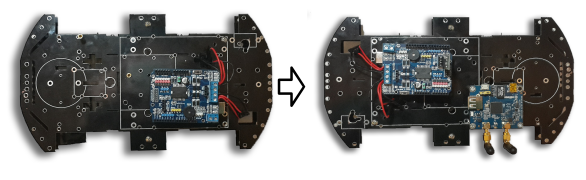
\includegraphics[width=1\linewidth]{build2.png}
\caption{Building Process 2}
\end{figure}
\end{frame}

\begin{frame}{Car Building Process}
The fourth step is to connect the HD Camera to the chassis. In the fifth step, the wheels are finally
mounted and the car is ready.
\begin{figure}[h]
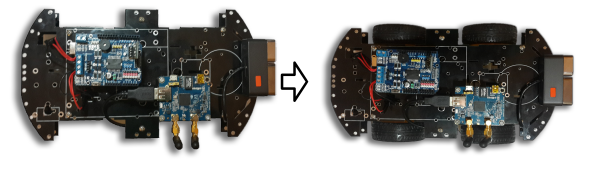
\includegraphics[width=1\linewidth]{build3.png}
\caption{Building Process 3}
\end{figure}
\end{frame}

	


%----------------------------------------

\begin{frame}{Arduino Programming Language}
\begin{block}{}
$\star$ Open-source Arduino Software (IDE)\\
\vspace{0.2cm}
$\star$ It is easy to write code and upload it to the board.\\
\vspace{0.2cm}
$\star$ The environment is written in Java.\\
\vspace{0.2cm}
$\star$ This software can be used with any Arduino board.
\end{block}
\end{frame}

\begin{frame}{Arduino Programming Language}
\begin{columns}[c] 
\column{.50\textwidth}
\begin{itemize}
\item[1.] It allows us to check the Arduino code for errors.
\item[2.] It allows us to execute our Arduino code and upload to board.
\end{itemize}
\column{.50\textwidth}
\begin{figure}
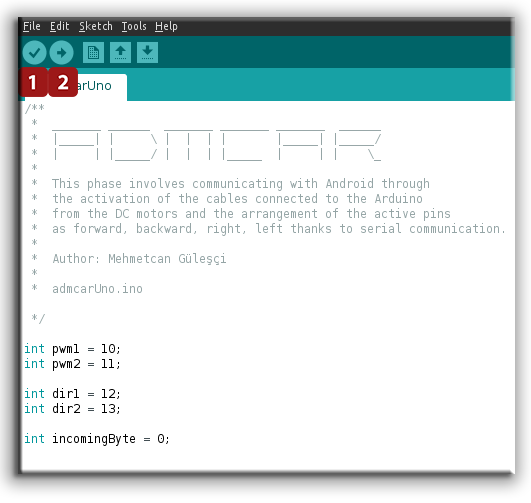
\includegraphics[width=1\linewidth]{update_execute.png}
\caption{Arduino Usage}
\end{figure}
\end{columns}
\end{frame}

\defverbatim[colored]\lstI{
\begin{lstlisting}[language=C++,basicstyle=\ttfamily,keywordstyle=\color{red}]
// Initialize variables
int pwm1 = 10;
int pwm2 = 11;

int dir1 = 12;
int dir2 = 13;

int incomingByte = 0;
\end{lstlisting}
}

\defverbatim[colored]\lstII{
\begin{lstlisting}[language=Java,basicstyle=\ttfamily,keywordstyle=\color{red}]
void setup()
{
  pinMode(pwm1, OUTPUT);
  pinMode(pwm1, OUTPUT);
  pinMode(dir1, OUTPUT);
  pinMode(dir2, OUTPUT);

  digitalWrite(pwm1, LOW);
  digitalWrite(pwm2, LOW);
  digitalWrite(dir1, LOW);
  digitalWrite(dir2, LOW);

  Serial.begin(9600);
}
\end{lstlisting}
}

\defverbatim[colored]\lstIII{
\begin{lstlisting}[language=Java,basicstyle=\ttfamily,keywordstyle=\color{red}]
void MotorKontrol(int mdir1, int mdir2, int pwmSpeed)
{
  digitalWrite(dir1, mdir1);
  digitalWrite(dir2, mdir2);
  analogWrite(pwm1, pwmSpeed);
  analogWrite(pwm2, pwmSpeed);
}
\end{lstlisting}
}

\defverbatim[colored]\lstIIII{
\begin{lstlisting}[language=Java,basicstyle=\ttfamily,keywordstyle=\color{red}]
    if (incomingByte == 10){ 
      MotorKontrol(HIGH, HIGH, 170); // Forward 
    }
    else if (incomingByte == 20){ 
      MotorKontrol(LOW, LOW, 170); // Backward
    }
    else if (incomingByte == 30){ 
      MotorKontrol(HIGH, LOW, 170); // Left
    }
    else if (incomingByte == 40){ 
      MotorKontrol(LOW, HIGH, 170); // Right
    }
    else{ // Stop if another data comes
      MotorKontrol(LOW, LOW, 0);
    }
\end{lstlisting}
}

\begin{frame}{Arduino Code}{Initialize variables}
\begin{columns}[c] 
\column{.50\textwidth}
\begin{block}{}
\lstI
\end{block}
\column{.50\textwidth}
\begin{block}{}
\lstII
\end{block}
\end{columns}
\end{frame}

\begin{frame}{Arduino Code}{Direction - Speed}
\begin{block}{}
\lstIII
\end{block}
\end{frame}

\begin{frame}{Arduino Code}{loop()}
\begin{block}{}
\lstIIII
\end{block}
\end{frame}



%----------------------------------------

\begin{frame}{Android Code Flows}{Bluetooth.java}
{\color{Red}{\textbf{Step 1 }}} Take our phone's bluetooth\\
\vspace{0.3cm}
{\color{Red}{\textbf{Step 2 }}} If you have a bluetooth but it is not open, request to connect.\\
\vspace{0.3cm}
{\color{Red}{\textbf{Step 3 }}} Take paired devices\\
\vspace{0.3cm}
{\color{Red}{\textbf{Step 4 }}} Method that allows us to select desired devices to connect.\\
\vspace{0.3cm}
{\color{Red}{\textbf{Step 5 }}} We get the mac address, the last 17 characters in the view.\\
\vspace{0.3cm}
{\color{Red}{\textbf{Step 6 }}} We define an intent to start a new activity.\\
\vspace{0.3cm}
{\color{Red}{\textbf{Step 7 }}} Start the activity.
\end{frame}

\begin{frame}{Android Code Flows}{MjpegStream.java}
{\color{Red}{\textbf{Step 1 }}} Mjpeg Input Stream which is not natively supported by Android is defined with 4 methods \texttt{getEndOfSequence}, \texttt{getStartOfSequence}, \texttt{parseContentLength} and r\texttt{eadFrame}.\\
\vspace{0.3cm}
{\color{Red}{\textbf{Step 2 }}} URI - \texttt{http://192.168.1.1:8080/?action=stream}\\
\begin{center}
\( Http Client \stackrel[Response]{Request}{{\Large \rightleftarrows}} Http Service \)\\
\end{center}
\vspace{0.3cm}
{\color{Red}{\textbf{Step 3 }}} Buffered Input Stream is created to read and skip many bytes at a time. So it prevents the cache memory from freezing.\\
\vspace{0.3cm}
{\color{Red}{\textbf{Step 4 }}} Data Input Stream is created. It lets an application read primitive Java data types from an underlying input stream in a machine - independent way.\\
\vspace{0.3cm}
{\color{Red}{\textbf{Step 5 }}} The Mjpeg Stream constructor is created to be called in the Car Activity class.
\end{frame}


\defverbatim[colored]\carActivity{
\begin{lstlisting}[language=Java,basicstyle=\ttfamily,keywordstyle=\color{red}]
Bitmap bitmap; // This is used in getting a video stream
Canvas canvas;

canvas.drawBitmap (bitmap, null, new Rect(0, 0, 
				  canvas.getWidth(), 
				  canvas.getHeight()), 
				  null) ;
\end{lstlisting}
}

\begin{frame}{Android Code Flows}{CarActivity.java}
{\color{Red}{\textbf{Step 1 }}} Sockets are created to send a data or connect to it.\\
\vspace{0.3cm}
{\color{Red}{\textbf{Step 2 }}} Bluetooth sockets are defined for each forward, backward, left and right buttons to provide motion.\\
\vspace{0.3cm}
{\color{Red}{\textbf{Step 3 }}} The surface create method created by the Surface.Holder Callback calls the mjpeg stream constructor we created in the previous class.\\
\vspace{0.3cm}
{\color{Red}{\textbf{Step 4 }}} Through the collaboration of the Canvas and Bitmap classes defined in it, the full size image becomes active.\\
\vspace{0.3cm}
\carActivity
\end{frame}


\begin{frame}{User Interface}
The application starts with the \textbf{intro picture.} Then the \textbf{second intent} comes out. This one requires connecting to the Bluetooth.
\vspace{0.2cm}
\begin{center}
$\vimage{intro.png}\vpointer
\vimage{blue_opt.png}$
\end{center}
\end{frame}

\begin{frame}{User Interface}
After the Bluetooth request has come out and when we click \texttt{No} option, the right window pops up and we get the warning of \texttt{'Paired devices not found. Be sure bluetooth connection is open.'}.
\vspace{0.2cm}
\begin{center}
$\vimage{blue_opt.png}\vpointer
\vimage{2.png}$
\end{center}
\end{frame}

\begin{frame}{User Interface}
In the Bluetooth permission request, if you press \texttt{Yes} and then press the \texttt{List} button, we will see the list of paired devices.
\vspace{0.2cm}
\begin{center}
$\vimage{blue_opt.png}\vpointer
\vimage{blue_yes.png}$
\end{center}
\end{frame}

\begin{frame}{User Interface}
As a final, when you click to bluetooth you are connected in, you will see the last intent to control the car. In this last intent, besides the view of the camera, it will be possible to control the car with the buttons.\\
\vspace{0.2cm}
\begin{center}
$\vimage{blue_yes.png}\vpointer
\vimage{main_screen.png}$
\end{center}
\end{frame}


%----------------------------------------

\begin{frame}{Class Diagrams}{Splash Activity}
This class that provides image transition time with the help of threads.
\begin{figure}
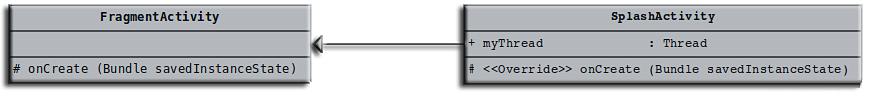
\includegraphics[width=1\linewidth]{Splash_class_diagram2.png}
\caption{Intro Screen Class Diagram}
\end{figure}
\end{frame}

\begin{frame}{Class Diagrams}{Bluetooth List}
It is a class that provides Bluetooth access to the Bluetooth feature of the phone with the help of Bluetooth adapters and makes some kind of communication with the Arduino Bluetooth via the Sockets.
\begin{figure}
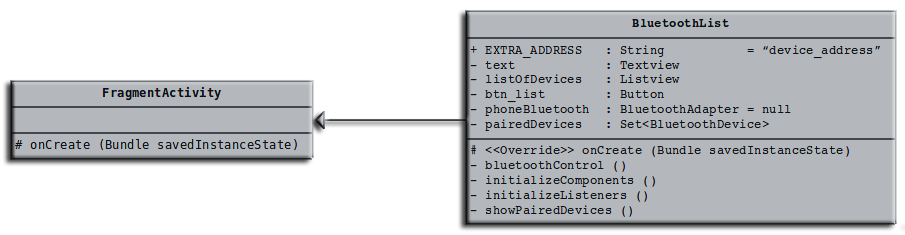
\includegraphics[width=1\linewidth]{Bluetooth_class_diagram2.png}
\caption{Bluetooth Class Diagram}
\end{figure}
\end{frame}


\begin{frame}{Class Diagrams}{Mjpeg Stream}
This one contains classes that control the camera, including video stream. Basically, everything is managed from the MjpegStream, it’s a view specialized to deal with Mjpeg video stream format, because Android doesn’t support natively this format.
\begin{figure}
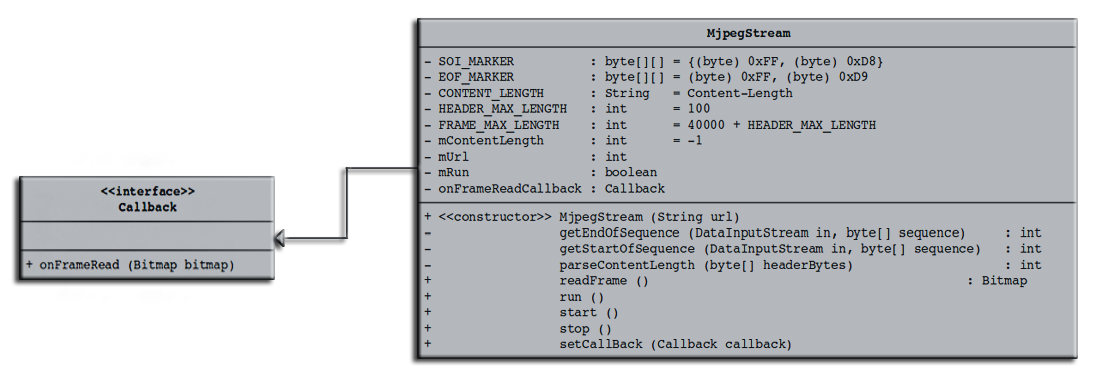
\includegraphics[width=1\linewidth]{Camera_class_diagram2.png}
\caption{Camera Class Diagram}
\end{figure}
\end{frame}


\begin{frame}{Class Diagrams}{Car Activity}
This class contains all classes in relationship with the car. The Car class is basically a controller for the car, it’s this class that will control the direction via bluetooth sockets and monitor the live video stream.
\begin{figure}
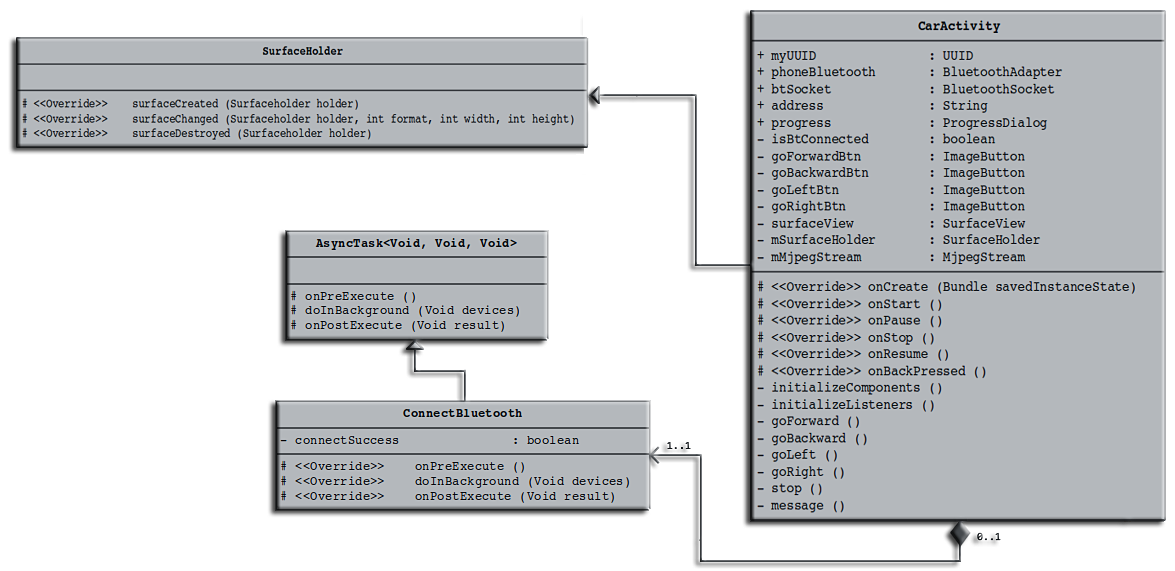
\includegraphics[width=1\linewidth]{Car_class_diagram2.png}
\caption{Car Activity Class Diagram}
\end{figure}
\end{frame}



%----------------------------------------

\begin{frame}{Use Case Diagrams}
To describe the system functionalities, we use the UML Use case diagrams. The Use Cases diagrams
illustrated below show the actors that show also which kind of action they can use.
This is the first version of the system, which can basically only move, the details about all the possible movements are described too.
\begin{figure}
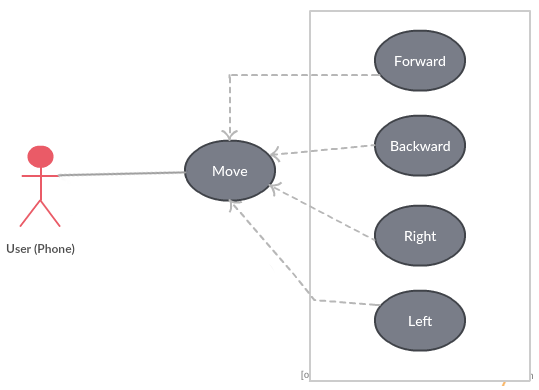
\includegraphics[width=0.6\linewidth]{RobotUML_V1.png}
\caption{Robot UML V1}
\end{figure}
\end{frame}
\begin{frame}
The second version is a major release of the system because we will reach our goal that is to have a video stream on the phone and control the car almost in real time with good performances.
\begin{figure}
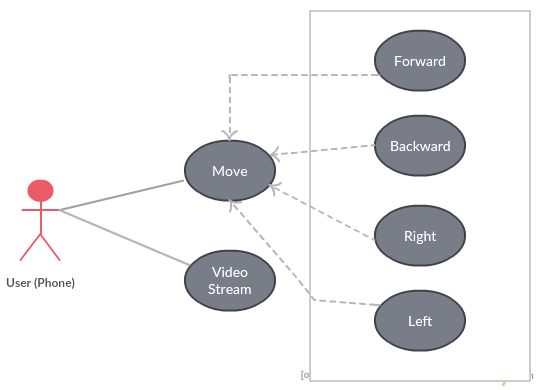
\includegraphics[width=0.6\linewidth]{RobotUML_V2.png}
\caption{Robot UML V2}
\end{figure}
\end{frame}


%----------------------------------------


%\subsection{Limitations of the system}
%\begin{frame}{Limitations of the system}
%\end{frame}


\begin{frame}{User profile}
\begin{block}{Who can use this application ?}
The users that will be play with the system could be child or adults, they just\\ \vspace{0.2cm}
have to know how to use a smartphone, launch an application and push some\\ \vspace{0.2cm} buttons. There is no really limitation about the age while they know how to use\\ \vspace{0.2cm} the phone.
\end{block}
\end{frame}


\begin{frame}{Strengths}
\begin{itemize}
\item The project works, we are able to do what we wanted.
\vspace{0.2cm}
\item The source code for both Android and Arduino is commented, well explained and documented with
external documents.
\vspace{0.2cm}
\item All the source code and the documentation are available for future usages for other people and free. (Git)
\vspace{0.2cm}
\item Good and speed video stream.
\vspace{0.2cm}
\item With the video streaming width designed to fill the user’s phone screen, the user will be able to control the car comfortably.
\vspace{0.2cm}
\item It connects to Bluetooth without difficulty and never breaks unless we are away from a certain distance.
\end{itemize}
\end{frame}

\begin{frame}{Weaknesses}
\begin{itemize}
\item The product needs two separated power sources.
\vspace{0.2cm}
\item Sometimes WiFi can shut down automatically. In this case, the video is freezing because WiFi is off.
\vspace{0.2cm}
\item Really short range with video stream. ( 8 meters)
\end{itemize}

\end{frame}


\begin{frame}{Suggested improvements (Future of system)}
\begin{itemize}
\item Use external antenna for greater range.
\vspace{0.1cm}
\item Use only one source of power, so use the big battery used by the motor for both motor and Arduino
using the regulator.
\vspace{0.1cm}
\item Study and fix bugs on the applications.
\vspace{0.1cm}
\item Improve the Android application to be able to get the video stream and the car control after lost them (out of range) automatically.
\vspace{0.1cm}
\item Add sounds to warn the user on some events such as “out of range”, “video lost”, etc.
\vspace{0.1cm}
\item Improve the application with new modules such as distance detection using sensor.
\vspace{0.1cm}
\item Improve Android application with a different way to control the car using sensors instead of buttons and propose the choice to the user between both.
\vspace{0.1cm}
\item Some sensors of the Arduino can be added to bring joy to the car. (honk-buzzer, distance-ultrasonic, headlights-lamp sensor etc.).
\end{itemize}

\end{frame}


%----------------------------------------


\begin{frame}{TIME TABLE AND WORK SCHEDULE}
\begin{figure}
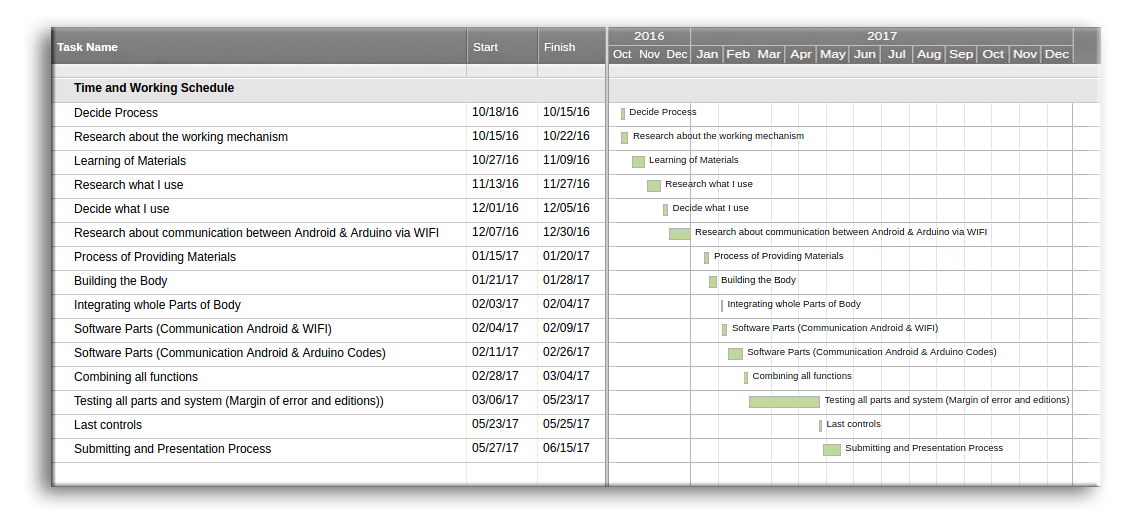
\includegraphics[width=1\linewidth]{ganttChart.png}
\caption{Time Table and Work Schedule}
\end{figure}
\end{frame}


%----------------------------------------


\begin{frame}{REFERENCES}
\begin{thebibliography}{9}
\setbeamertemplate{bibliography item}[online]
%\bibitem{A} {\scriptsize \url{http://www.robotistan.com/arduino-smd-l298-cift-motor-surucu-shield-arduino-motor-shield#}}
%\bibitem{A} {\footnotesize \url{https://gelecegiyazanlar.turkcell.com.tr/konu/arduino/egitim/arduino-201/bluetooth-ile-iletisim}}
\bibitem{A} {\scriptsize \url{http://stackoverflow.com/questions/4032391/android-bluetooth-where-can-i-get-uuid}}
\bibitem{A} {\scriptsize \url{http://www.robotiksistem.com/dc_motor_ozellikleri.html}}
\bibitem{A} {\scriptsize \url{http://electrotech.tv/arduinoya-giris-arduino-nedir-ne-degildir-1bolum/}}
\bibitem{A} {\scriptsize \url{http://android.serverbox.ch/?p=1039}}
\bibitem{A} {\scriptsize \url{http://stackoverflow.com/questions/3205191/android-and-mjpeg}}
\bibitem{A} {\scriptsize \url{http://forum.arduino.cc/}}
\bibitem{A} {\scriptsize \url{https://sites.google.com/site/androidhowto/how-to-1/display-a-web-page}}
\bibitem{A} {\scriptsize \url{http://www.bluecove.org/bluecove/apidocs/javax/bluetooth/UUID.html}}

\end{thebibliography}
\end{frame}


%------------------------------------------------


\begin{frame}
\Huge{\centerline{The End}}
\end{frame}


\end{document}

